\begin{frame}{Theory: Topological insulator}
	2005 Kane and Mele found another class of material: \\the topological insulator (TI).
	\\
	\begin{columns}
		\begin{column}<2->{0.33\linewidth}
			spin-orbit coupling
		\end{column}
		\hspace{-1cm}
		\begin{column}<3->{0.33\linewidth}
			$\rightarrow$ band inversion
		\end{column}
		\hspace{-1.2cm}
		\begin{column}<4->{0.33\linewidth}
			$\rightarrow$ Dirac cone
		\end{column}
	\end{columns}
	\begin{columns}
		\begin{column}<4->{.5\linewidth}
			\begin{figure}
				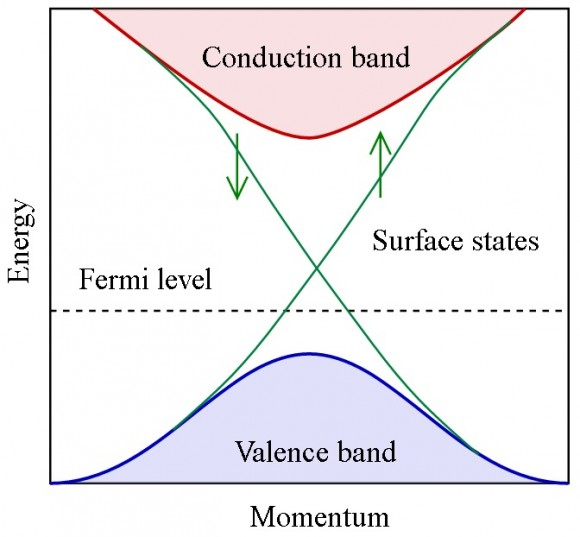
\includegraphics[width=\textwidth]{andere_bilder/band_structure_top_insulator}
			\end{figure}
		\end{column}
		\begin{column}{.5\linewidth}
			\begin{block}<5->{2D TI: }
			have quantum spin edge states found in graphene and HgTe quantum wells.
			\end{block}
			\begin{block}<6->{3D TI: }
			strong and weak ones \\
			HgTe is semi metal but under strain $\Gamma_6$ and $\Gamma_8$ bands can close up at Fermi level. 
			\end{block}
		\end{column}
	\end{columns}
	\note{Besides from insulators and conductors, Kane and Mele 2005 found another class of material which is the so-called topological insulator. Most of the unusual properties come from the including of the spin-orbit coupling. This produces the spin-momentum locking mentioned earlier and can lead to band inversion. The spin-momentum locking and time-reversal symmetry prevent backscattering, because for two opposite momentums, the spin is also opposite and the states interfere destructively.  In other words, the surface states are protected by time-reversal symmetry. If the surface states close up because of band inversion then a so-called Dirac cone arises like seen in this picture from wikipedia. Here we see the momentum plotted against the energy near Fermi level. The blue line is the valence band and the red one is the conduction band. The surface states in green have a spin locked to their momentum and are forming a Dirac cone because their bands are inverted. \\	
	In 2D there were found topological surface states in graphene and HgTe quantum wells which are called Quantum spin edge states based on the Quantum spin hall effect. These quantum wells have non-trivial topological surface states under a certain critical thickness but become trivial insulators as soon as they pass this critical thickness.
	3D topological insulators are distinguishable into strong and weak topological insulators where the number of dirac cones is odd for strong and even for weak ones. HgTe normally is a semi metal but under strain its $\Gamma_6$ and $\Gamma_8$ bands can close up at Fermi level, which means its surface states become topological.}
\end{frame}

\begin{frame}{Theory: Crystal and surface description part 1}

	\begin{block}{Translation vector: $\boldsymbol{R}_i = x_i \boldsymbol{a}_1 + y_i \boldsymbol{a}_2 + z_i \boldsymbol{a}_3$}
		contains basis for lattice forming a unit cell. \\
		Smallest primitive unit cell is the Wigner Seitz cell.
	\end{block}
	\begin{columns}
		\begin{column}<2->{0.3\linewidth}
			Bravais lattice  
		\end{column}
	\end{columns}
	\begin{columns}
		\begin{column}<3->{0.5\linewidth}
			fcc lattice with two atomic basis 
		\end{column}
		\hspace{-1cm}
		\begin{column}<4->{0.55\linewidth}
			$\rightarrow$ diamond or zinc-blende structure 
		\end{column}
	\end{columns}
	\hfill
	\begin{columns}<5->
		\begin{column}{.25\linewidth}
			\centering
			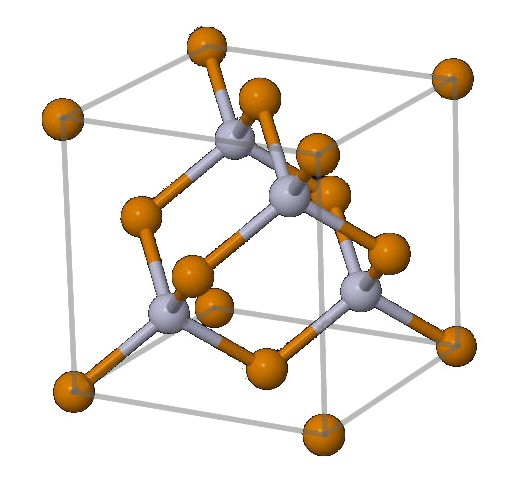
\includegraphics[width=\linewidth]{andere_bilder/zinc_blende}
		\end{column}
%		\hspace{-.7cm}
		\begin{column}{.25\linewidth} 
		\scriptsize{
			\centering
			\begin{tabular}{c c c c} 
				\hline
				& \textbf{x} & \textbf{y} & \textbf{z}\\ 
				\hline 
				\vspace{0.2cm} 
				$\boldsymbol{a}_1$ & $0$ & $\frac{a}{2}$ & $\frac{a}{2}$ \\
				\vspace{0.2cm}
				$\boldsymbol{a}_2$ & $\frac{a}{2}$ & $0$ & $\frac{a}{2}$ \\
				\vspace{0.2cm}
				$\boldsymbol{a}_3$ & $\frac{a}{2}$ & $\frac{a}{2}$ & $0$ \\
%			\end{tabular}	
%		\end{minipage}
%		\\
%		\begin{column}[c]{.33\linewidth}
%			\begin{tabular}{c c c c} 
%				\hline
%				& \textbf{x} & \textbf{y} & \textbf{z}\\ 
				\hline 
				\vspace{0.2cm}
				Te & $0$ & $0$ & $0$ \\
				\vspace{0.2cm}
				Hg & $\frac{a}{4}$ & $\frac{a}{4}$ & $\frac{a}{4}$
			\end{tabular}
		}
		\end{column}
		\begin{column}<6->{.5\linewidth}
			\begin{minipage}{\linewidth}
			Miller indices: $(hkl)$
			\begin{equation*}
			h : k : l = \frac{1}{x} : \frac{1}{y} : \frac{1}{z}
			\end{equation*}
			\end{minipage}
			\\
			\begin{minipage}{\linewidth}
			\centering
			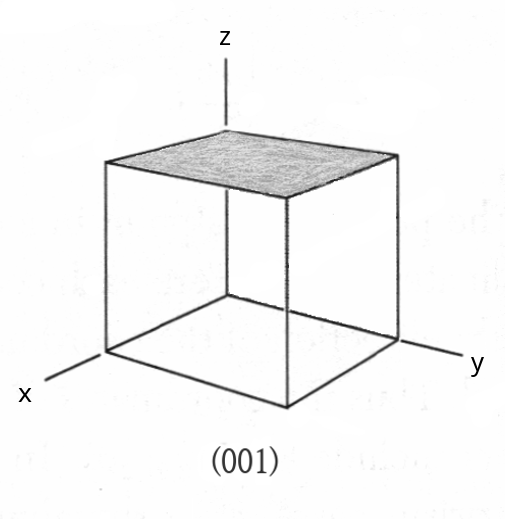
\includegraphics[width=.5\linewidth]{extrabilder_fuer_vortrag/millersche_indizes_001}
			\end{minipage}
		\end{column}
	\end{columns}
	\note{The atoms of a crystal maintain a symmetric pattern that repeats itself in our case into the three spatial dimensions. In order to describe that crystalline structure, we make use of the translation vector R i which contains information about the coordinates x, y and z of an atom i and the primitive translation vectors a one, a two and a three that form a so-called unit cell. It is a primitive unit cell, if it contains the least possible amount of atoms. The smallest primitive unit cell is called Wigner Seitz cell and has one single atom in its center. \\
	The lattices which are generated by R i are called Bravais lattice and in three dimensional space there are 14 of them. The face-centered cubic (fcc) lattice with two atomic basis is the structure needed here. If the atoms are of the same species, then it is called a diamond structure, if the atoms are of a different kind of species, it's called a zinc-blende structure. The latter is the one for mercury telluride. Here you can see the basis of it and a picture of a cubic. This is the basis for the bulk calculations. \\
	Surfaces however are described by the Miller indices h, k and l which are related to numbers x, y and z, and if one multiplies the basis vector with those numbers, the basis vectors touch the surface. If the basis vector can never touch the surface, then the Miller index is set to zero. This is why this plane (picture) is the (001) plane. }
\end{frame}

\begin{frame}{Theory: Crystal and surface description part 2}
	Basis for (001) direction of zinc-blende structure: 
	\begin{columns}
		\hspace{-1cm}
		\begin{column}<2->{.25\linewidth}
			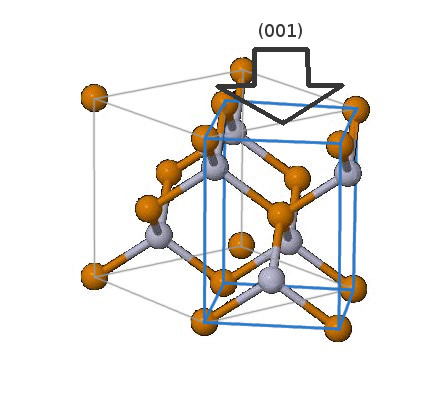
\includegraphics[width=1.2\linewidth]{andere_bilder/zinc_blende_45degree.jpg}
		\end{column}
		\hspace{-1cm}
		\begin{column}<2->{.2\linewidth}\scriptsize{
			\begin{tabular}{c c c c} 
				\hline
				& \textbf{x} & \textbf{y} & \textbf{z}\\ 
				\hline 
				\vspace{0.2cm} 
				$\boldsymbol{a}_1$ & $\frac{a}{\sqrt{2}}$  & $0$ & $0$ \\
				\vspace{0.2cm}
				$\boldsymbol{a}_2$ & $0$ & $\frac{a}{\sqrt{2}}$ & $0$ \\
				\vspace{0.2cm}
				$\boldsymbol{a}_3$ & $0$ & $0$ & $a$ 
			\end{tabular}
		}	
		\end{column}
		\begin{column}<2->{.3\linewidth}\scriptsize{
			\begin{tabular}{c c c c} 
				\hline
				& \textbf{x} & \textbf{y} & \textbf{z}\\ 
				\hline
				\vspace{0.2cm} 
				Te & $0$ & $0$ & $0$ \\
				\vspace{0.2cm}
				Hg & $\frac{a}{2\sqrt{2}}$ & $0$ & $\frac{a}{4}$ \\
				\vspace{0.2cm}
				Te & $\frac{a}{2\sqrt{2}}$ & $\frac{a}{2\sqrt{2}}$ & $\frac{a}{2}$ \\
				\vspace{0.2cm}
				Hg & $0$ & $\frac{a}{2\sqrt{2}}$ & $\frac{3a}{4}$
			\end{tabular}
		}
		\end{column}
	\end{columns}
	\begin{columns}
		\begin{column}<3->{.6\linewidth}
			Reciprocal lattice: $e^{i\boldsymbol{K}\boldsymbol{R}} = 1$\\
			$\boldsymbol{K}$ is reciprocal translation vector.\\
			First Brillouin zone (BZ) is Wigner Seitz cell for reciprocal space.\\
			Super symmetrical points:\vspace{-.3cm}
			\begin{align*}
			\overline{\Gamma}&= 0;&
			\overline{\text{J}} &= \frac{1}{2} \boldsymbol{b}_1 ;&
			\overline{\text{K}}&= \frac{1}{2} \boldsymbol{b}_1 + \frac{1}{2} \boldsymbol{b}_2 
			\end{align*}
		\end{column}
		\begin{column}<3->{.4\linewidth}
			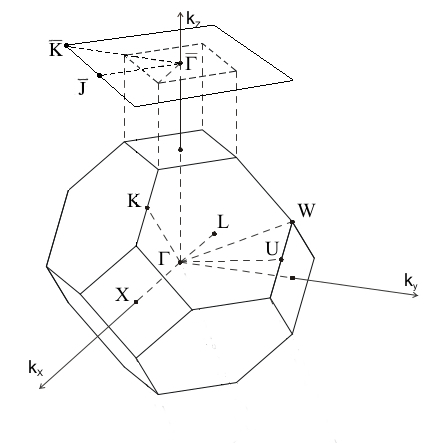
\includegraphics[width=\linewidth]{andere_bilder/brillouin_zone_001_2}
		\end{column}
	\end{columns}
	\note{For calculations in the (001) direction, it is convention to rotate the unit cell by 45 degrees which gives us another basis for HgTe.\\
	As we say before, the energy bands are obtained by observing the momentum with respect to the energy. The best way to do so is, to use the reciprocal lattice which is the Fourier transform of the real lattice with (formular with e function). K is the reciprocal translation vector with reciprocal lattice vectors b1, b2 and b3. The first Brillouin zone is the Wigner Seitz cell for the reciprocal space. It contains so-called high symmetry points, in the picture one can see a $\Gamma$ in the origin. Every other high symmetry point is indicated by Latin letters. The points with a bar on top are the high symmetry points for the 2D Brillouin zone which we will use for the surface calculations, in concrete: Gamma bar, J bar, K bar.}
\end{frame}

\begin{frame}{Theory: Surface modeling}
	\begin{columns}
		\begin{column}{.86\linewidth}
			\begin{block}{Termination}
				Two surfaces with symmetric Hg-Hg, Te-Te terminations or antisymmetric Te-Hg terminations.\\
				Add hydrogen atoms in order to saturate dangling bonds. 
			\end{block}
			\begin{block}<2->{Number of layers}
				Odd for symmetric, even for antisymmetric termination.\\
				Atoms with same $z$ component are in the same layer.\\
				I studied 3 different thicknesses for each termination.				
			\end{block}
			\begin{block}<3->{Supercell approach}
				Infinite repetition only possible in all directions.\\
				In order to avoid interactions between slabs in $k_z$ direction: add vacuum space. 
			\end{block}
		\end{column}
		\begin{column}<3->{0.14\linewidth} 
			\centering
			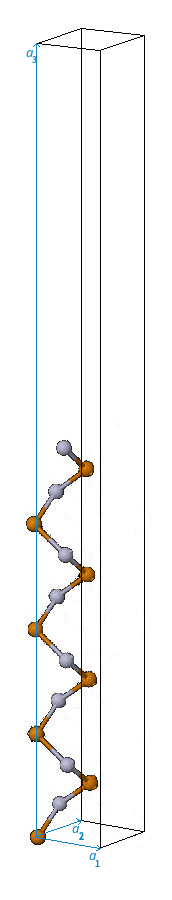
\includegraphics[width=\linewidth]{andere_bilder/hgte_16layer_supercell_2.jpg} 
		\end{column} 
	\end{columns}
	\note{Now I will talk about what we have to consider for simulating the surfaces in (001) direction. At first, there are different possible terminations at the top and the bottom surfaces. Either the terminations are symmetric Hg-Hg or Te-Te, or they are antisymmetric with Te-Hg. I also performed calculations with additional hydrogen atoms at one surface in order to saturate the dangling bonds (the unsatisfied valences on immobilized atoms). \\
	The number of layers corresponds to the kind of termination, it is odd for symmetric and even for antisymmetric ones. 
	In our case, one layer contains every atom with the same z component.
	And I studied three different numbers of layers or thicknesses for each kind of termination. \\
	Our approach for simulating the surface in one direction contains an infinite repetition in the other two directions. Unfortunately FHI-aims can only repeat in all three directions. In order to avoid interactions between the slabs in k z direction and simulate a surface, one adds vacuum space to the unit cell. This is called the supercell approach. The supercell for 16 layers is illustrated in the picture at the right, where a1 and a2 are as explained before, but a3 is not only as long as the slab is thick, but also contains additional vacuum space.}
\end{frame}

\begin{frame}{Theory: Density functional theory (DFT)}	
	\begin{block}{First Hohenberg-Kohn Theorem:}
		$\rho(\boldsymbol{r})$ can be uniquely converted into the $V_\text{ext}(\boldsymbol{r})$
	\end{block}
	\begin{block}<2->{Second Hohenberg-Kohn Theorem:}
		Ground state energy can be expressed in a density functional: \vspace{-.35cm}
		\begin{equation*}
		E^{\text{HK}}[\rho(\boldsymbol{r}); v_{\text{ext}}(\boldsymbol{r})] = 
		T_0 [\rho] + V_\text{H} [\rho] + \int v_{\text{ext}}(\boldsymbol{r}) \rho(\boldsymbol{r}) \diff \boldsymbol{r} + E_{\text{xc}} [\rho]
		\end{equation*}
	\end{block}
	\begin{block}<3->{Kohn-Sham equation}
		Minimizing $E^{\text{HK}}$ $\rightarrow$ Kohn-Sham eigenfunctions $\phi_i(\boldsymbol{r})$: \vspace{-.35cm}
%		 and $\rho(\boldsymbol{r}) = \sum_i |\boldsymbol{p}hi_i(\boldsymbol{r})|^2$:
		\begin{equation*} 
		E_0 [\rho_0] = E_{\text{nucl}} + E_{\text{kin}} + E_\text{H} + E_{\text{xc}} 
		\end{equation*}
	\end{block}
	\begin{block}<4->{Perdew-Burke-Ernzerhof (PBE) functional} \vspace{-.15cm}
		\begin{equation*}
		E_{\text{xc}}^{\text{PBE}} = \int \diff^3 r \rho(\boldsymbol{r}) 
		\,\epsilon_{\text{xc}}^{\text{PBE}} (r_s (\boldsymbol{r}), s(\boldsymbol{r}), \zeta(\boldsymbol{r}))
		\end{equation*}
	\end{block}
	\note{The density functional theory was first introduced by
		W.Kohn et al. They found that the ground-state energy of a quantum
		mechanical system can be represented by a density functional.
		For wave function of a many-body Schrödinger equation with an Hamiltonian containing the kinetic energy, the Coulomb potential between the particles, in our case electrons, and the external Potential which is the nuclei, one can define a one-body ground states density rho. The first Hohenberg-Kohn Theorem then says that rho can be uniquely converted into the external potential and vice versa. (In other words, for one given V ext, there exists specifically one rho) \\
		The second Hohenberg-Kohn Theorem says that the ground state energy of such a many-body system can be expressed in a density functional. T zero thereby is the kinetic energy for a system of non-interacting electrons, the rest builds the Hohenberg-Kohn potential which contains the Hartree potenial and the exchange-correlation function. Note that the small v ext is the external potential just for one electron but contains all protons of the nucleus.\\
		By minimzing this density functional we get the Kohn-Sham eigenfunctions phi i and the Kohn-Sham equation.	The exchange correlation functional can not be determined exactly, so there are several approximations been done. One of them is the Perdew-Burke-Ernzerhof functional, short: PBE. It is a semilocal-density functional,
		which does not only dependent on the density at a certain position. This means it is  better for big molecules or systems in comparison to the LDA functional, which is only local (as the name local density approach indicates). }
\end{frame}

\begin{frame}{Theory: Spin-orbit coupling}
	\begin{columns}<2->
		\begin{column}{.5\linewidth}
			Dirac equation:
		\end{column}\hspace{-3.3cm}
		\begin{column}{.7\linewidth}
			\begin{equation*}
			\left(
			c \boldsymbol\alpha \cdot \boldsymbol{p} + c^2(\beta - 1) + V
			\right) \Psi = \epsilon \Psi
			\end{equation*}
		\end{column}
	\end{columns}
	\begin{columns}<3->
		\begin{column}{.6\linewidth}
			Separate $\Psi$ into two spinors:
		\end{column}\hspace{-5cm}
		\begin{column}{.4\linewidth}
			\begin{equation*}
			\Psi = 
			\begin{pmatrix}
			\Psi_\text{L} \\ \Psi_\text{S}
			\end{pmatrix}
			\end{equation*}	
		\end{column}
	\end{columns}
	\begin{columns}<4->
		\begin{column}{\linewidth}
			Substitute and dissolve:
			\begin{align*}
			\left(
			\boldsymbol{p} \frac{c^2}{2c^2 + \epsilon - V} \boldsymbol{p} 
			+ i \boldsymbol{p} \frac{c^2}{2c^2 + \epsilon - V} \times \boldsymbol{p} \cdot \boldsymbol{\sigma} 
			+ V 
			\right) \Psi_\text{L} 
			&= \epsilon \Psi_\text{L}	
			\end{align*}
		\end{column}
	\end{columns}
	\vspace{.3cm}
	\begin{columns}<6->
		\begin{column}{\linewidth}
			First part with $V$ is relativistic Schrödinger equation.
		\end{column}
	\end{columns}
	\begin{columns}<7->
		\begin{column}{\linewidth}
			Expanding in $\frac{\epsilon - V}{2c^2}$ in zeroth order gives non-relativistic Schrödinger equation. 
		\end{column}
	\end{columns}
	\begin{columns}<8->
		\begin{column}{\linewidth}
			Expanding just second part in first order gives:
			\begin{equation*}
			V_{\text{SOC}} = \frac{i}{4c^2} \boldsymbol{p} V \times \boldsymbol{p} \cdot \boldsymbol{\sigma}
			\end{equation*}
		\end{column}
	\end{columns}
	\note{ The spin-orbit interaction is the interaction between a particles spin and its motion. The Dirac equation explains why it should be included in the Schrödinger equation.
	Here we see the Dirac equation for electrons, where alpha contains in the top at right and in the bottom at left a sigma vector with all three Pauli matrices, and beta is the matrix containing the 2D basis matrix in the left upper part and minus 2D basis matrix in the right lower part. p is the momentum. 
	Then we separate the wave function Psi into two spinors, large for the one that positive energies, means it represents the electrons, and is dominant for the non-relativistic limit, and small for negative energies, means positrons, which disappear in the non-relativistic limit. By substituting this into the Dirac equation and dissolve the two coupled equations we get this Schrödinger like equation. \\
	The first part together with the V is the relativistic Schrödinger equation. By expanding it in epsilon minus V over 2 times c squared in zeroth order and then sets epsilon to zero, it gives us the non-relativistic Schrödinger equation. 
	By expanding only the second part of that equation above in first order, one gets the spin-orbit coupling potential. \\
	If a structure contains heavy elements, like HgTe, it is necessary to include this potential since spin-orbit interaction also affects valence electrons. This is not the case for light elements. 
	The SOC calculations are performed by FHI-aims after the self consistency cycle converged. 
	In the band structure it can cause band splitting on degenerated bands. }
\end{frame}

%%% Local Variables:
%%% mode: latex
%%% TeX-master: "main_BA2_Vortrag.tex"
%%% End: